\title{Resampling Spectra While Maintaining Diagonal Covariance}
\author{Stephen Bailey}
\date{\today}

\documentclass[12pt]{article}

\usepackage{graphicx}

\newcommand{\C}{\mathbf{C}}
\newcommand{\Ci}{\mathbf{C}^{-1}}
\newcommand{\R}{\mathbf{R}}
\newcommand{\A}{\mathbf{A}}
\newcommand{\N}{\mathbf{N}}
\newcommand{\Q}{\mathbf{Q}}
\newcommand{\f}{\mathbf{f}}
\newcommand{\m}{\mathbf{m}}

\begin{document}
\maketitle

\abstract{We discuss methods for resampling and coadding spectra while
maintaining diagonal covariance in the final spectra.}

\section{Introduction}

When analyzing spectra, any model fits should be transformed into the original
wavelength sampling of the data rather than resampling the
spectra into the model space.  Similarly, if you can avoid it, you shouldn't
coadd unaligned spectra into a single spectrum on a different wavelength
grid.  Instead, you should simultaneously fit any models directly
to the original input spectra.

This isn't always practical.  The extra hassle and
computational time of
``forward modeling'' may not be worth the statistical gains of doing
everything perfectly optimally.  Resampling and fully propagating the
covariance may be similarly burdensome.
But what you absolutely should
\emph{not} do is resample (or coadd) the spectra onto a different
wavelength grid---thus introducing covariance---and then pretend
that the newly introduced off-diagonal covariance doesn't exist and
ignore it.

Unfortunately this latter case is what many spectral analyses do,
{\it e.g.,}~any analysis based upon SDSS/BOSS coadded spectra is effectively
doing this.  There is covariance between the spectral bins that is neither
propagated nor reported, and any $\chi^2$ fit of a model to that data is
at some level incorrect.

This note explores a middle ground---how to resample spectra onto a new
wavelength grid while simultaneously maintaining diagonal
covariance to simplify the error propagation.  This enables coadds without
covariance between bins and resampling unaligned spectra onto a common
wavelength grid without off-diagonal covariance.  It makes use of the
``resolution matrix'' of Bolton \& Schlegel (2010) to diagonalize the
resampled spectra without employing the full ``spectroperfectionism''
extraction methodology.
We explore 3 cases: resampling a single
spectrum, coadding unaligned spectra, and resampling a set of covariant
unaligned spectra onto a common diagonally covariant wavelength grid.

Before you object that this is impossible --- we agree that there is no
free lunch.  Transforming to a diagonal basis moves the bookkeeping out
of the covariance matrix and into the resolution matrix that prescribes
how to move from the original wavelength sampling into the diagonalized
resampled space.  This transformation
contains the same information as the covariant resampled basis.
Any loss of information comes from the resampling itself,
not the diagonalization of the errors.
You can't get around that.  But you can achieve sampling that is both
convenient and diagonally covariant.  This note shows you how.

%-------------------------------------------------------------------------
\section{Resampling a single spectrum}
\label{sec:single_spec}

Given a spectrum $\f$ with non-covariant errors $\sigma_i$ sampled at
wavelengths $\lambda_i$, we wish to resample the spectrum at a different
set of wavelengths $\lambda_j^\prime$.
We solve this by modeling a linear transform from the new
sampling back to the original sampling:
\begin{equation}
    \f = \A \f^\prime
\end{equation}
Note that this is {\em not} $\f^\prime = \A \f$ --- we are seeking a model
that can be resampled to the data rather than resampling the data to the
model wavelengths.
$\A$ can be any linear transform from the new $\lambda^\prime$ sampling
back to the original $\lambda$ sampling, e.g. linear interpolation or
B-splines.  For the examples in this note we will use the simplest case
of linear interpolation.

The inverse covariance matrix of $\f^\prime$ is
\begin{equation}
    \Ci = \A^T \N^{-1} \A
\end{equation}
where $\N^{-1}$ is the diagonal weights matrix formed by $\sigma_i^{-2}$.
The solution to $\f^\prime$ is
\begin{eqnarray}
    \f^\prime & = &  (\A^T \N^{-1} \A)^{-1} \A^T \N^{-1} \f \\
              & = & \C \A^T \N^{-1} \f    \label{eq:solve_fprime}
\end{eqnarray}

The covariance $\C$ will have off-diagonal terms introduced by the
wavelength resampling.
Following Bolton \& Schlegel (2010), we can transform $\C$ and
$\f^\prime$ into a diagonal basis with a ``resolution matrix'' $\R$
\begin{eqnarray}
    \tilde{\C} & = & \R \C \R^T \\
    \tilde{\f}^\prime & = & \R \f^\prime
\end{eqnarray}
such that $\tilde{\f}^\prime$ is a spectrum sampled at $\lambda^\prime$ with
{\em diagonal} covariance $\tilde{\C}$.
Appendix~\ref{sec:solve_R} shows the derivation of $\R$ given $\Ci$.
For now, note that $\R$ is \emph{not} just an eigenbasis rotation,
which in general is a non-local transformation.  $\R$ maintains the
locality of spectral features while also diagonalizing the errors.

The $\chi^2$ of a model $\m$ is equivalent in either the original covariant
sampling or the diagonalized sampling by also transforming $\m$ with $\R$:

\begin{eqnarray}
    \chi^2  & = & (\f - \m)^T \Ci (\f - \m) \\
%             & = & (\f - \m)^T \R^T \tilde \Ci \R (\f - \m) \\
%             & = & (\R \f - \R \m)^T \tilde \Ci (\R \f - \R \m) \\
            & = & (\tilde \f - \R \m)^T \tilde \Ci (\tilde \f - \R \m) \\
            & = & \sum_i {\left( \tilde \f - \R \m \right)_i^2 \over \tilde C_{ii}}
\end{eqnarray}

There is no free lunch --- while $\tilde \Ci$ is now simpler to track
than $\C$, the off-diagonal bookkeeping has moved into $\R$.
This may still be beneficial, e.g.~visualizations of $\tilde \f$ are
not confused by the ringing of covariant bins.

\subsection{Example: Resampling a single spectrum}

\begin{figure}[t]
\centering
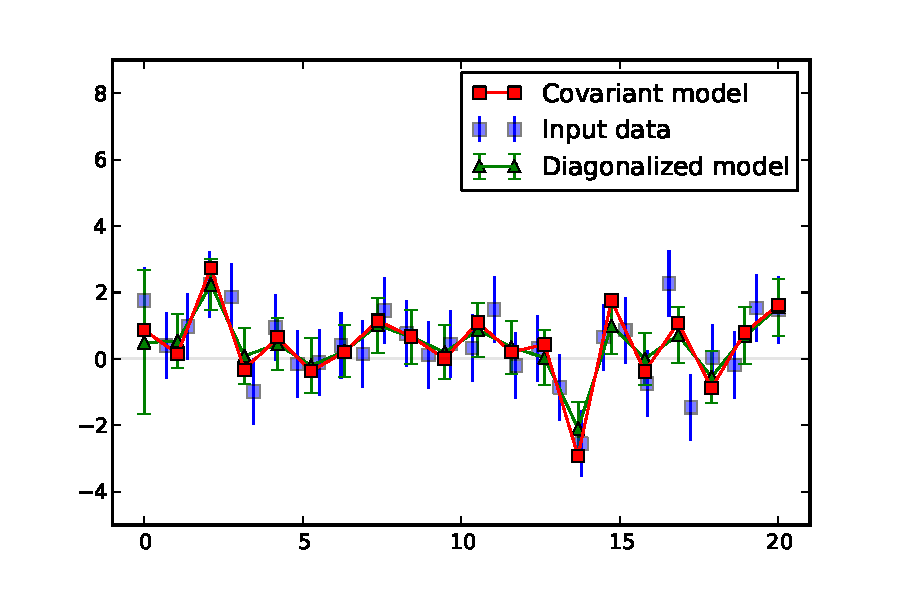
\includegraphics[width=0.8\textwidth]{plots/single_spec_1.pdf}
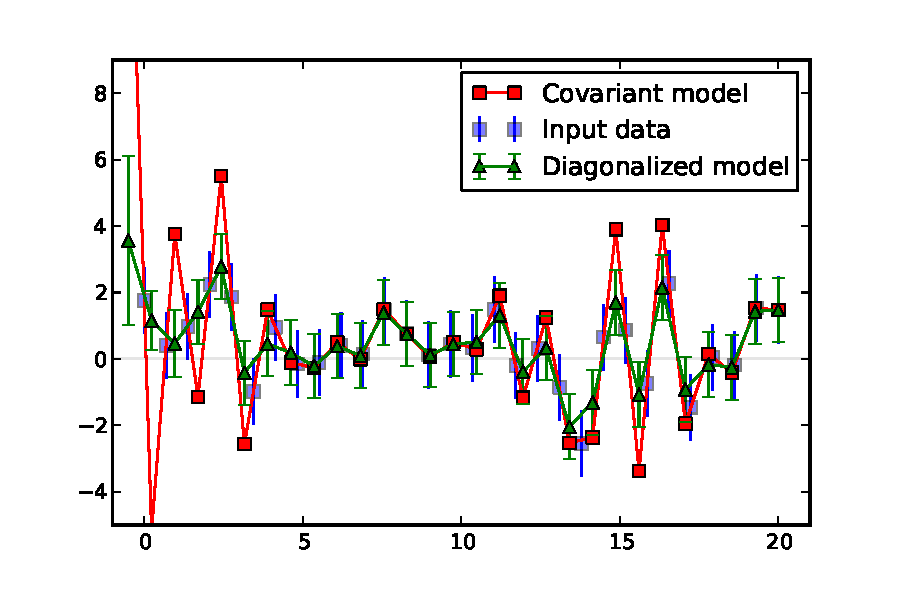
\includegraphics[width=0.8\textwidth]{plots/single_spec_2.pdf}
\caption{
Examples of resampling a spectrum (blue) to a different
wavelength grid (red) and then diagonalizing the covariance (green).
The ringing in the red spectra is due to covariance between bins
that is removed by the diagonalization process.
}
\label{fig:resample_spectrum}
\end{figure}

Figure~\ref{fig:resample_spectrum} shows examples of resampling a single
input spectrum (blue squares) to a new wavelength grid (red squares)
for two different final wavelength grids.
The amount of covariance introduced is heavily dependent upon the
phasing of the input and output grids.  The green triangles show the
final spectrum resulting from diagonalizing the covariance.
Higher order interpolations such as cubic B-splines would have
less covariant ringing at the expense of spreading that covariance
over multiple bins.  The same procedure can be applied to diagonalize
any interpolation that can be parameterized as a matrix operation
$\f = \A \f^\prime$.

%-------------------------------------------------------------------------
\section{Coadding spectra}
\label{sec:coadd}

The same method can be used to coadd multiple spectra that are not natively
aligned on the same wavelength grid.
\begin{equation}
    \mathbf{g} = \mathbf{B} \f_\mathrm{coadd}
\end{equation}
where $\mathbf{g}$ is the concatenation of the individual input spectra,
and $\mathbf{B}$
is the combined transformation matrix from the new sampling to the original
individual samplings.  i.e. for $n$ spectra,
\begin{equation}
    \left[ \begin{array}{c}
        \f_1 \\
        \f_2 \\
        \vdots \\
        \f_n \\
    \end{array}
    \right] = \left[ \begin{array}{c}
        \A_1 \\
        \A_2 \\
        \vdots \\
        \A_n \\
    \end{array}
    \right] \f_\mathrm{coadd}
\end{equation}

The calculation proceeds as in the previous section, finding a resolution
matrix $\R$ that transforms the inverse covariance
$\Ci = \mathbf{B}^T \N^{-1} \mathbf{B}$ into a diagonal basis.

\subsection{Example: coadding spectra}

\begin{figure}[t]
\centering
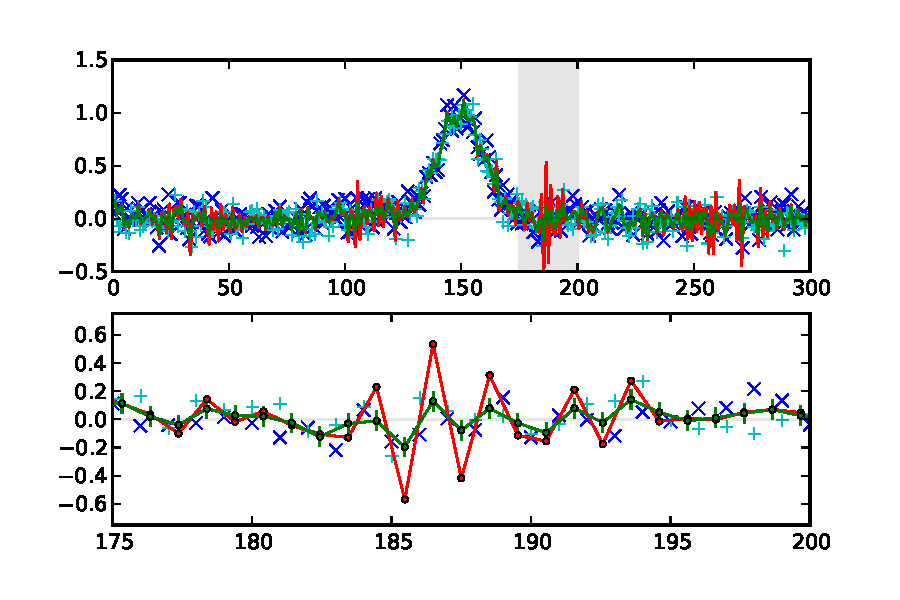
\includegraphics{plots/coadd_spectra.pdf}
\caption{
Example of coadding unaligned spectra onto a new wavelength grid.
Red shows the initial covariant resampling; green shows the diagonalized
coadded spectrum.  The bottom plot shows a zoom of the highlighted region
of the upper plot.  The ringing in the red spectrum is due to covariance
between the bins that is removed by the diagonalization procedure.
}
\label{fig:coadd_spectra}
\end{figure}

Figure~\ref{fig:coadd_spectra} shows the results for coadding unaligned
spectra onto a new common wavelength grid.
Red shows the initial covariant resampling; green shows the diagonalized
coadded spectrum.  The original covariant coadd shows large oscillations
at certain wavelengths where the coadd overfits the data.  The diagonalized
coadded spectrum does not have this problem.

%-------------------------------------------------------------------------
\section{Resampling covariant spectra}

The same method can be used to simultaneously resample multiple
covariant spectra onto a common wavelength grid.

\begin{eqnarray}
    \left[ \begin{array}{c}
        \f_1 \\
        \f_2 \\
        \vdots \\
        \f_n \\
    \end{array}
    \right] & = & \left[ \begin{array}{cccc}
        \A_1 \\
        & \A_2 \\
        & & \ddots \\
        & & & \A_n \\
    \end{array}
    \right] \left[ \begin{array}{c}
        \f_1^\prime \\
        \f_2^\prime \\
        \vdots \\
        \f_n^\prime \\
    \end{array}    
    \right] \\
    \mathbf{g} & = & \mathbf{B} \mathbf{g}^\prime
\end{eqnarray}
In this case the $\f_i^\prime$ spectra are {\em different} spectra that
we wish to sample onto the same wavelength grid, {\it e.g.}, IFU spectra
of a galaxy for a data cube.  If the various spectra $\f_i$ are not noise
correlated with each other,
then the resampling of $\f_i = \A_i \f_i^\prime$ proceeds identically to
section \ref{sec:single_spec}.  If they are noise correlated, then the
math is still the same as equation~\ref{eq:solve_fprime}
but now $\N^{-1}$ is the full inverse noise covariance
of the multiple input spectra rather than a diagonal matrix.

\subsection{Example: resampling covariant spectra}

\begin{figure}[t]
\centering
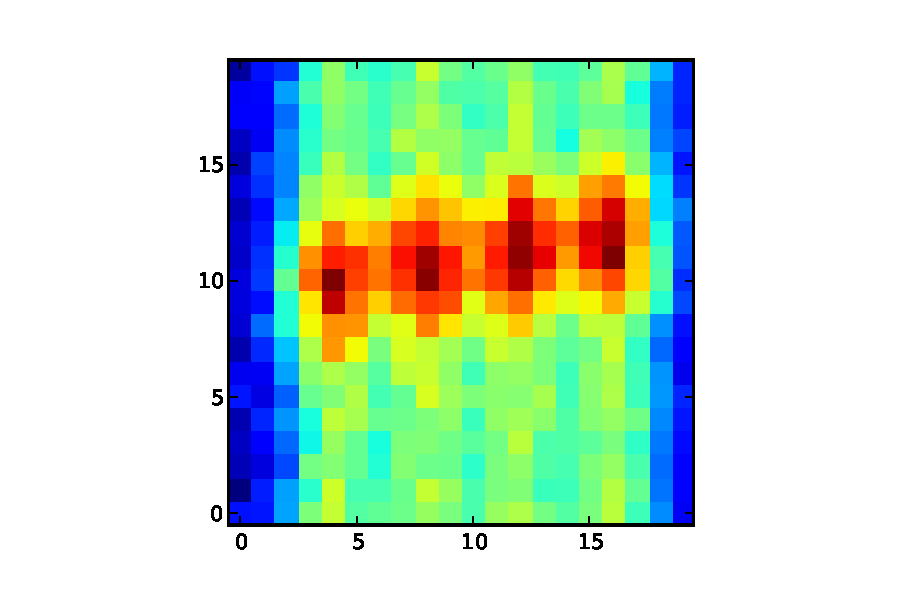
\includegraphics[height=0.4\textheight]{plots/multispec_img.pdf}
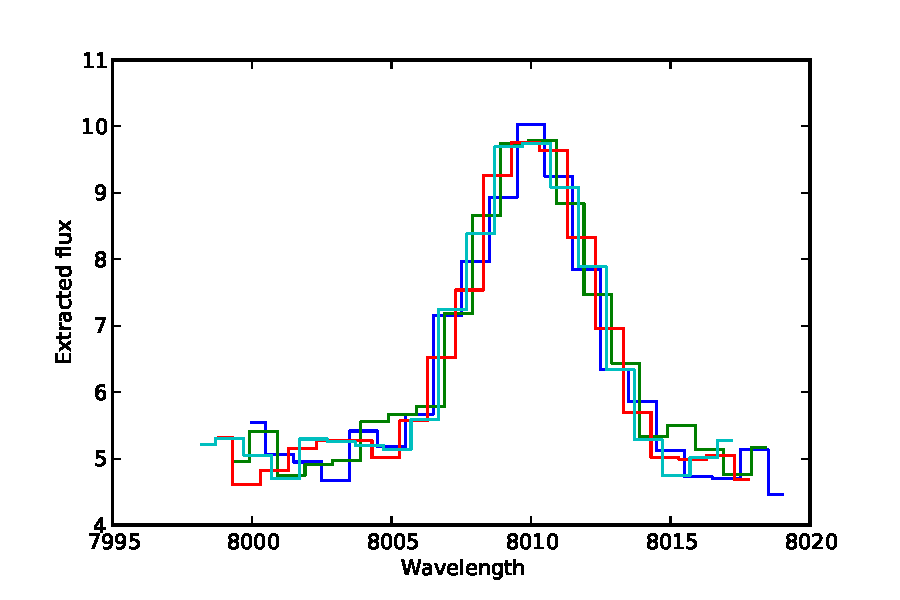
\includegraphics[height=0.4\textheight]{plots/multispec_extract.pdf}
\caption{
Top: Example image with 4 spectra that are not wavelength aligned in the
native CCD row sampling.
Bottom: Example row-by-row extraction of those spectra.
}
\label{fig:multispec_img}
\end{figure}

\begin{figure}[t]
\centering
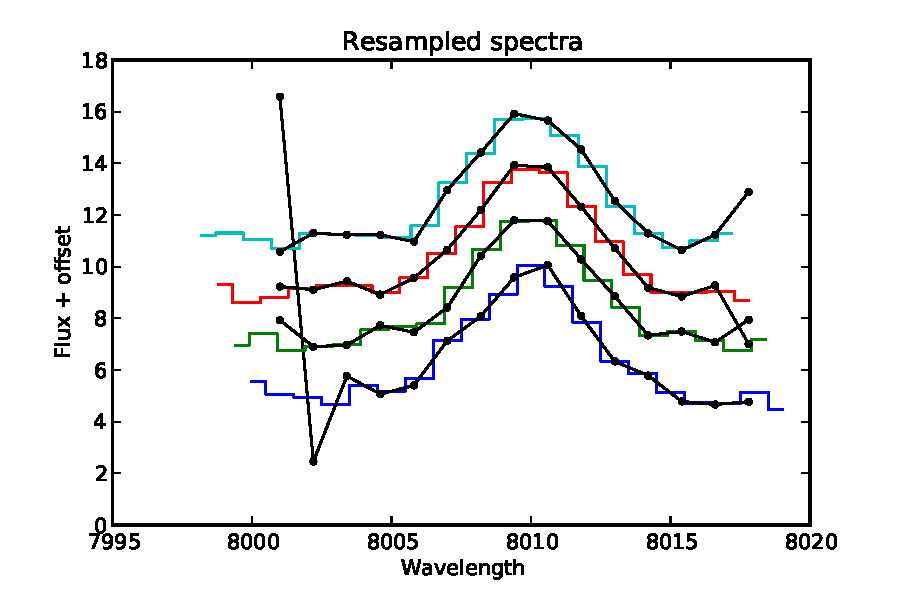
\includegraphics[height=0.4\textheight]{plots/multispec_resample.pdf}
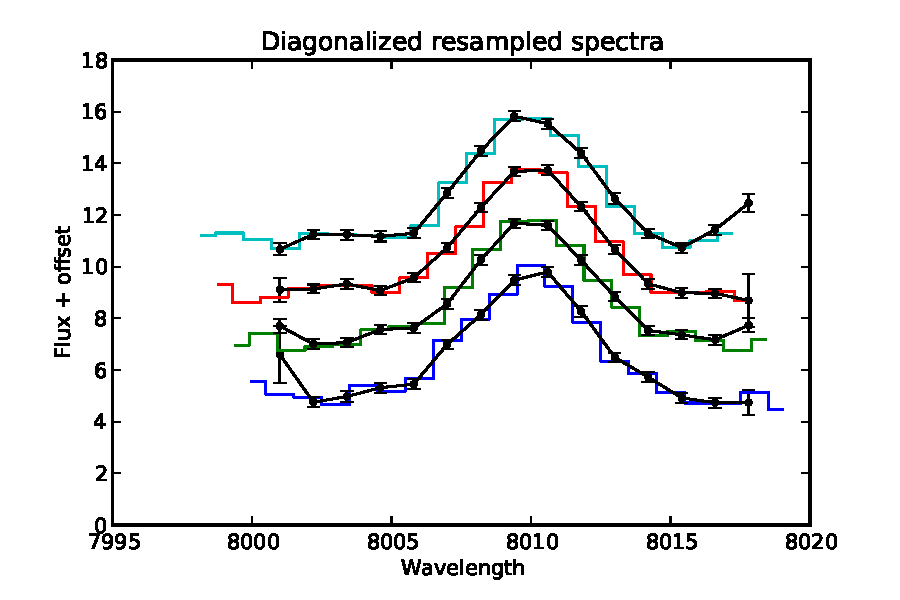
\includegraphics[height=0.4\textheight]{plots/multispec_diag.pdf}
\caption{
Top: resampled spectra with covariant ringing.
Bottom: simultaneously diagonalized resampled spectra.
}
\label{fig:multispec_resample}
\end{figure}

\begin{figure}[t]
\centering
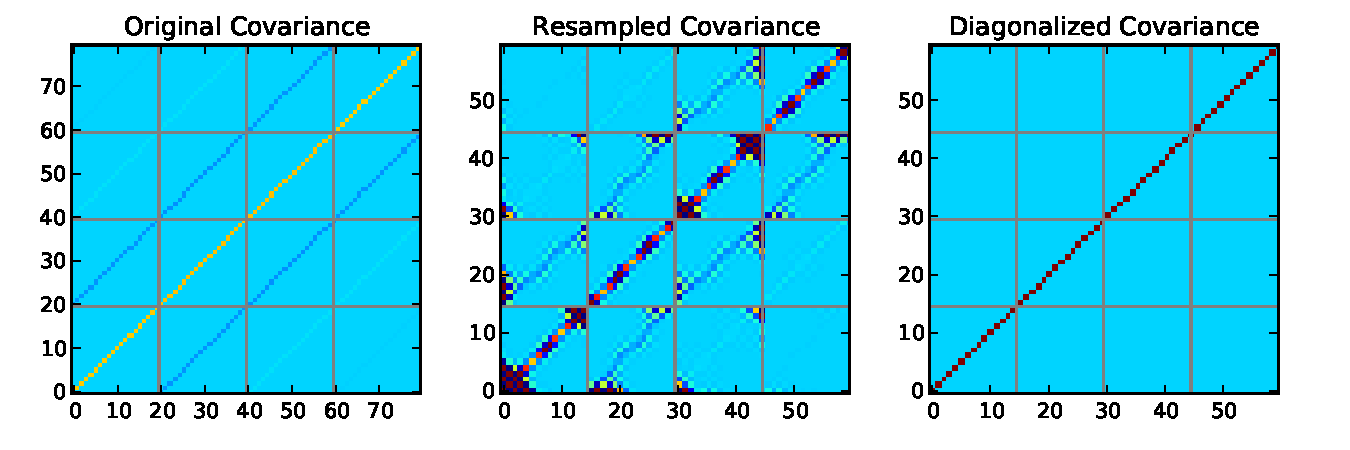
\includegraphics[width=\textwidth]{plots/multispec_cov.pdf}
\caption{
Covariance of the original row-by-row extraction (left),
the simultaneously resampled spectra (middle),
and the final diagonalized covariance (right).
The horizontal and vertical gray lines indicate the boundaries
between spectra.
}
\label{fig:multispec_cov}
\end{figure}


Figure~\ref{fig:multispec_img} shows example data for coadding multiple
unaligned spectra onto a common wavelength grid.  The upper image shows
four spectra on a CCD with wavelength dispersion running vertically.
The spectra overlap and thus are covariant when extracted, and
the emission line is offset between the spectra showing that the native
CCD row sampling is not on the same wavelength grid for each spectrum.
The bottom figure shows the row-by-row extraction of those spectra on
the native wavelength grid for each spectrum, showing that the bins do
not align.

Figure~\ref{fig:multispec_resample} (top) shows the results of resampling
these spectra onto a common wavelength grid.  Even when propagating the
original extraction covariance, the resampling introduces additional
covariance.  The bottom figure shows the diagonalization of the resampled
spectra with less ringing.

The covariance matrices are shown in
figure~\ref{fig:multispec_cov}.  The left plot shows the covariance
of the original row-by-row extractions; the middle plot shows the extra
covariance introduced by resampling; and the right plot shows the final
diagonalized covariance.

\section{Conclusion}

We end by re-iterating the admonition from the introduction:
if you can forward model, do that.  If you can't, don't ignore
off-diagonal covariances.  This note shows a method with examples
that allows you to resample and coadd spectra onto a new wavelength
grid while also maintaining the desirable property of diagonal covariance.

I thank Julien Guy and Adam Bolton for useful conversations directly
relevant to this work.


%-------------------------------------------------------------------------
\appendix
\section{Solving for the resolution matrix $\R$}
\label{sec:solve_R}

This appendix shows how to solve for $\R$ given inverse covariance $\Ci$,
following Bolton \& Schlegel (2010) equations 10 through 16 with a few more 
steps filled in.

We seek to find a transformation $\R$ such that $\tilde \C = \R \C \R^T$
is the diagonal covariance of a transformed spectrum $\tilde \f = \R \f$.
Start by finding the symmetric square root $\Q$ of $\Ci$ such that
$\Ci = \Q\Q$.  This can be found by eigen-decomposing $\Ci$ and
reconstructing $\Q$ with the square root of the eigenvalues:
\begin{eqnarray}
    \Ci & = & \mathbf{V} \mathbf{\Sigma}^{-1} \mathbf{V}^T \\
       & = & (\mathbf{V} \mathbf{\Sigma}^{-1/2} \mathbf{V}^T)
             (\mathbf{V} \mathbf{\Sigma}^{-1/2} \mathbf{V}^T) \\
    \Q & = &  \mathbf{V} \mathbf{\Sigma}^{-1/2} \mathbf{V}^T
\end{eqnarray}
Also note that $\C = \mathbf{V} \mathbf{\Sigma} \mathbf{V}^T$
and $\Q = \Q^T$.

Next, define a diagonal normalization matrix $\mathbf{S}$ with elements
\begin{equation}
    S_{ii} = 1 / \sum_j Q_{ij}
    \label{eq:Sdef}
\end{equation}
and a resolution matrix
\begin{equation}
    \R = \mathbf{S} \Q .
    \label{eq:RSQ}
\end{equation}
Thus by construction,
\begin{eqnarray}
    \tilde \C & = & \R \C \R^T \\
              & = & (\mathbf{S} \Q)
                    (\mathbf{V} \mathbf{\Sigma} \mathbf{V}^T)
                    (\Q^T \mathbf{S}^T) \\
              & = & \mathbf{S}
                    (\mathbf{V} \mathbf{\Sigma}^{-1/2} \mathbf{V}^T)
                    (\mathbf{V} \mathbf{\Sigma} \mathbf{V}^T)
                    (\mathbf{V} \mathbf{\Sigma}^{-1/2} \mathbf{V}^T)
                    \mathbf{S} \\
              & = & \mathbf{S}^2 .
\end{eqnarray}
i.e.~$\tilde \C$ is a diagonal matrix giving the covariance of
$\tilde \f = \R \f$.

\subsection{Normalization of $\mathbf{S}$}

Note that any diagonal matrix $\mathbf{S}$ could be used in
equation~\ref{eq:RSQ} with the resulting transformed $\tilde \f$ having
diagonal variance $\mathbf{S}^2$.  The normalization choice in
equation~\ref{eq:Sdef} is what is proposed in Bolton \& Schlegel (2010),
but this is not the only choice.
It does have the desirable property of maintaining the locality of the
spectra\footnote{This is an emperical observation; I honestly don't see
why that is true from the math.},
i.e.~the resulting $\R$ acts like a convolution of the input
covariant spectra.

However, this normalization does \emph{not} conserve flux,
i.e.~$\sum \R \f \ne \sum \f$.  An alternate
normalization that \emph{does} conserve flux is
\begin{equation}
    S_{ii} = \sum_j Q^{-1}_{ij}
\end{equation}
We are exploring the consequences of using this alternate normalization.


\end{document}
